\section{Orientation}
In order to draw a \rubik{} on the screen there is to things which are needed; the position of each \cubie{} and the orientation of each \cubie{}.

A corner \cubie{} in a given \cubicle{} can ``sit'' in this \cubicle{} in one of three ways.
These different orientations can thereby be defined with an integer between 0 and 2.
0 if the primary \facelet{} is on the primary \face{}, 1 if the primary \facelet{} is on the secondary \face{}, and 2 if the primary \facelet{} is on the tertiary \face{}.
See the figure \ref{fig:orientation} for an illustration.

\begin{figure}[htb]
	\centering
		\subfloat[\myCaption{The white/blue/red corner is correctly oriented, which gives it the orientation value 0.}]{\label{fig:orientation:orientation0}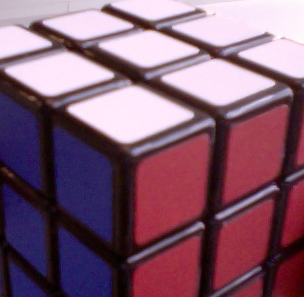
\includegraphics[width=0.28\textwidth]{input/pics/orientation0}}
		\hspace{0.02\textwidth}
		\subfloat[\myCaption{The white/blue/red corner is incorrectly oriented, the orientation value of this is 1 since the primary color is on a secondary face.}]{\label{fig:orientation:orientation1}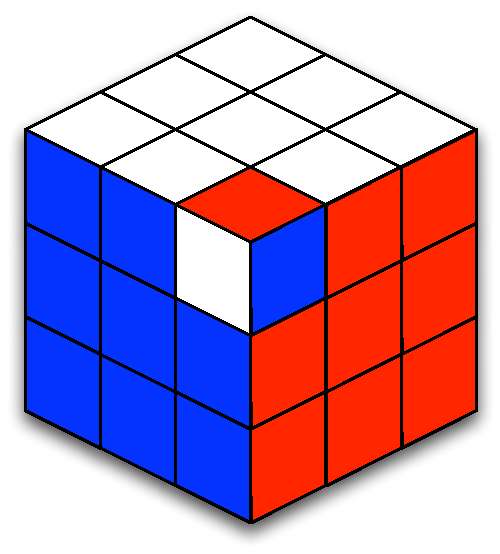
\includegraphics[width=0.28\textwidth]{input/pics/orientation1}}
		\hspace{0.02\textwidth}
		\subfloat[\myCaption{The white/blue/red corner is incorrectly oriented, the orientation value of this is 1 since the primary color is on a secondary face.}]{\label{fig:orientation:orientation2}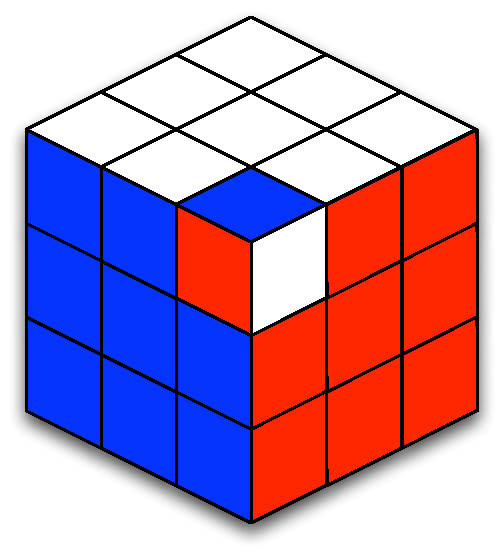
\includegraphics[width=0.28\textwidth]{input/pics/orientation2}}
		\caption{\myCaption{The three different orientation which the white/blue/red cubie can have.}}
		\label{fig:orientation}
\end{figure}

The orientation of a edge \cubie{} can be defined with a boolean value; either it is correctly oriented or it is not.
This is easiest to see when the \cubie{} is in the right position e.g.
If the white/blue edge \cubie{} is in its correct \cubicle{} then it is correctly oriented if the white \facelet{} is on the white \face{} and the blue \facelet{} is on the blue \face{}.
The orientation is wrongly oriented if the blue \facelet{} is on the white \face{} and the white \facelet{} is on the blue \face{}.

This raises the question: What is the orientation of a \cubie{} which is not in its correct \cubicle{}?
